\documentclass[tikz, xcolor=dvipsnames]{standalone}
\usepackage{amsmath}
\usepackage{xcolor}
\usetikzlibrary{arrows, automata, positioning, calc}
\begin{document}

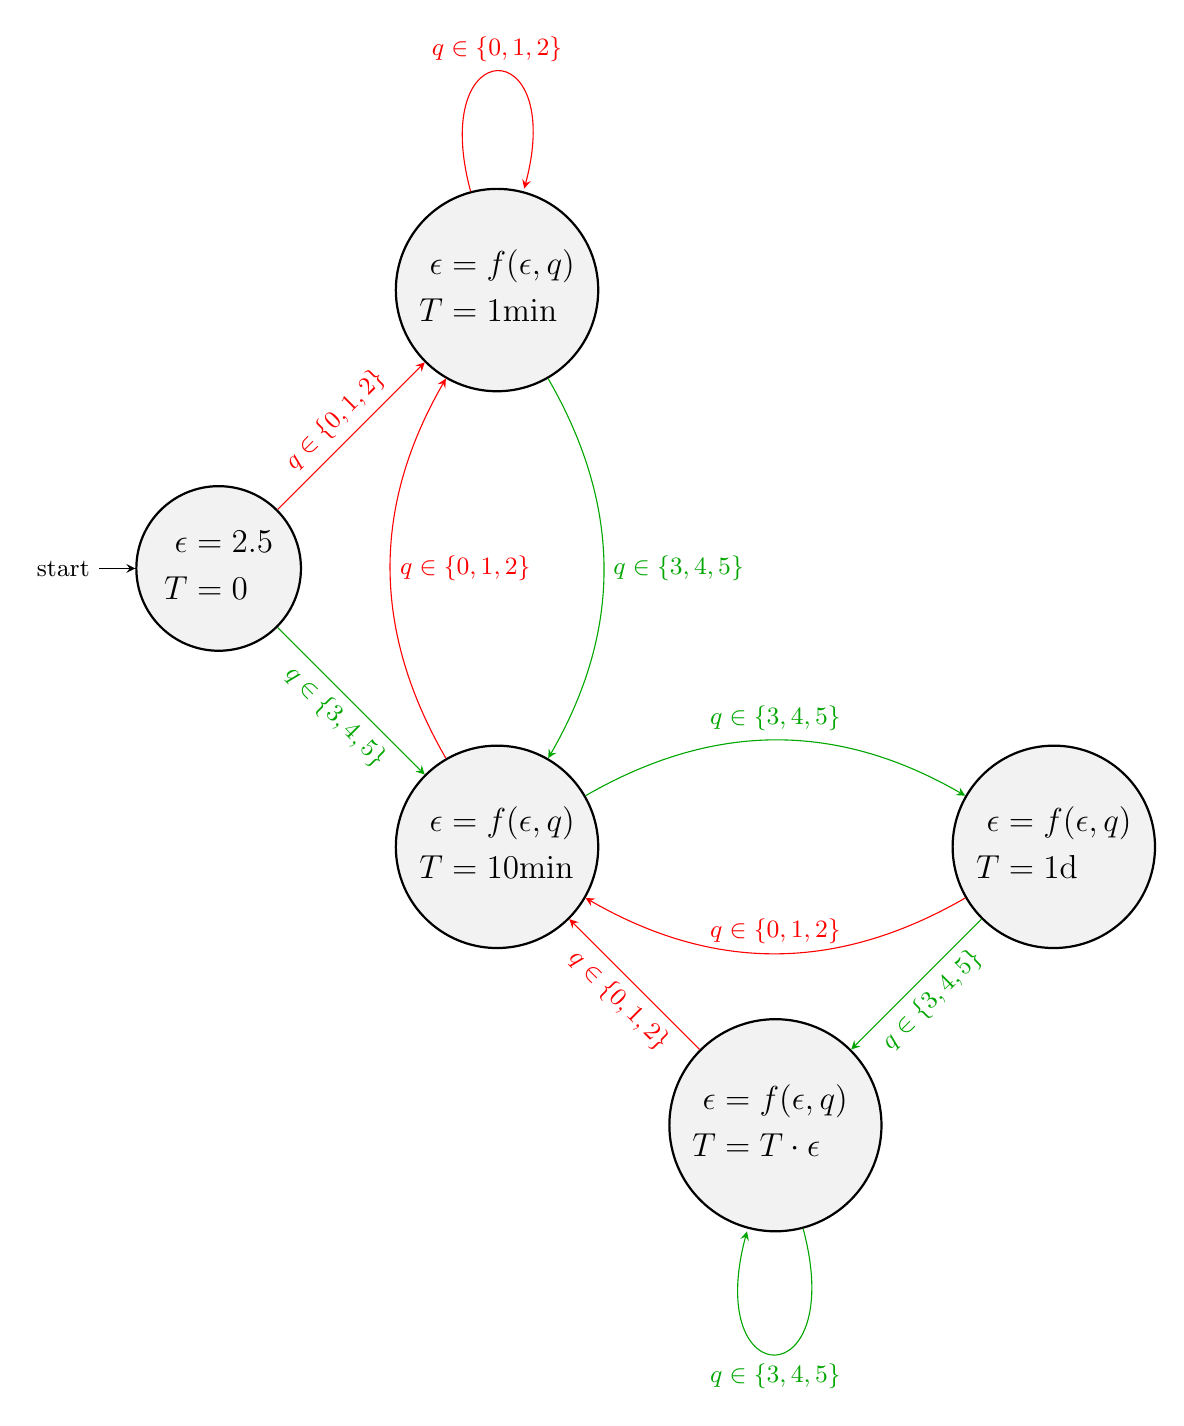
\begin{tikzpicture}[
    ->,  % makes the edges directed
    >=stealth,
    node distance=5cm, % specifies the minimum distance between two nodes. Change if necessary.
    every node/.style={font={\small}}, % sets the properties for each ’state’ node
    every state/.style={thick, fill=gray!10, font={\large}}, % sets the properties for each ’state’ node
    corr/.style={color=green!65!black},
    incorr/.style={color=red}
  ]

  \node[state, initial] (q1) {
    $\begin{aligned}
      \epsilon &= 2.5 \\
      T &= 0 \\
    \end{aligned}$
  };

  \node[state, above right of=q1] (q2) {
    $\begin{aligned}
      \epsilon &= f(\epsilon, q) \\
      T &= 1\text{min} \\
    \end{aligned}$
  };

  \node[state, below right of=q1] (q3) {
    $\begin{aligned}
      \epsilon &= f(\epsilon, q) \\
      T &= 10\text{min} \\
    \end{aligned}$
  };

  \node[state, below right of=q3, align=center] (q4) {
    $\begin{aligned}
      \epsilon &= f(\epsilon, q) \\
      T &= T \cdot \epsilon \\
    \end{aligned}$
  };

  \node[state, above right of=q4] (q5) {
    $\begin{aligned}
      \epsilon &= f(\epsilon, q) \\
      T &= 1\text{d} \\
    \end{aligned}$
  };

  \draw (q1) edge[incorr, sloped, anchor=center, above] node{$q \in \{0, 1, 2\}$} (q2);
  \draw (q2) edge[incorr, loop above] node{$q \in \{0, 1, 2\}$} (q2);
  \draw (q1) edge[corr, sloped, anchor=center, below] node{$q \in \{3, 4, 5\}$} (q3);
  \draw (q3) edge[incorr, bend left, right] node{$q \in \{0, 1, 2 \}$} (q2);
  \draw (q2) edge[corr, bend left, right] node{$q \in \{3, 4, 5 \}$} (q3);
  \draw (q3) edge[corr, bend left, above] node{$q \in \{3, 4, 5\} $} (q5);
  \draw (q5) edge[incorr, bend left, above] node{$q \in \{0, 1, 2\} $} (q3);
  \draw (q5) edge[corr, sloped, anchor=center, below] node{$q \in \{3, 4, 5\} $} (q4);
  \draw (q4) edge[incorr, sloped, anchor=center, below] node{$q \in \{0, 1, 2\} $} (q3);
  \draw (q4) edge[corr, loop below] node{$q \in \{3, 4, 5\}$} (q4);

\end{tikzpicture}

\end{document}
